\documentclass[a4paper,11pt]{article}
\usepackage[utf8]{inputenc}
\usepackage[spanish]{babel}
\usepackage{hyperref}
\usepackage{enumerate}
\usepackage{amssymb, amsmath, amsbsy}
\usepackage{sectsty} %Este paquete se usa para poder cambiar el tamaño de las letras de los encabezados, y que no salgan demasiado grandes.
\usepackage[pdftex]{graphicx}
\begin{document}
\allsectionsfont{\normalsize}
\title{Cálculo de una instalación telesilla biplaza}
\author{Francisco Javier Romero Porras}
\maketitle
\begin{abstract}
Este es un trabajo que nos permite ver un ejemplo de como se debe proyectar un telesilla, de modalidad biplaza, de panza fija, para turistas no esquiadores. El trabajo se incluirá en el siguiente repositorio de git:\\
\url{https://github.com/fjromeropo/proyecto_final}
\end{abstract}
\textbf{Palabras claves:} proyecto, telesilla, biplaza, pilona, cable, perfil.
\tableofcontents
\part{Introducción}
El objetivo del artículo es ejemplificar como debe proyectarse un telesilla biplaza, de panza fija, para turistas no esquiadores, entre dos puntos distantes 550 m y con un desnivel total de 150 m. Se considerarán, además, las siguientes características para hacer el dimensionado de la instalación:\\
\begin{itemize}
\item La capacidad de la instalación será de $C=702 viajeros/hora$
\item La altura total de silla y pasajero es de 3.50 m
\item Se considera que no hay nieve, pero deben tenerse en cuenta los efectos dinámicos.
\item La masa de la silla es de 60 kg (biplaza), y se considera un peso de 80 kg por viajero.
\item Los volantes de ambas estaciones se encuentran a 4.00 m sobre el terreno.
\item El tipo de cable es de 6x36+1 Warrington - Seale
\item Por razones de explotación la propiedad impone las siguientes condiciones:
\begin{itemize}
\item La altura máxima de apoyos será de 12 m
\item El diámetro máximo del cable será de 32 mm
\item Se procurará que no se produzcan cambios de signo de la carga sobre los apoyos al pasar de la situación de cargado a descargado.
\item El motor y contrapeso deben disponerse en la estación inferior.
\end{itemize}
\item Los cálculos generales se realizarán en cuatro hipótesis de carga:
\begin{enumerate}[a)]
\item Ramal ascendente cargado y descendente cargado.
\item Ramal ascendente cargado y descendente descargado.
\item Ramal ascendente descargado y descendente cargado.
\item Ramal ascendente descargado y descendente descargado.
\end{enumerate}
\end{itemize}
El perfil del terreno que vamos a usar en nuestro ejemplo vendrá dado por 22 pares de puntos que nos generarán un perfil longitudinal del telesilla. Estos pares de puntos vienen dados en la siguiente tabla:\\
\\
\begin{table} \centering
\begin{tabular}{|c|c|c|}
\hline
Perfil & Distancia al origen (m) & Cota (m)\\
\hline
0 & 0 & 0\\
\hline
1 & 25 & 2\\
\hline
2 & 50 & 10\\
\hline
3 & 75 & 20\\
\hline
4 & 100 & 30\\
\hline
5 & 125 & 38\\
\hline
6 & 150 & 45\\
\hline
7 & 175 & 55\\
\hline
8 & 200 & 65\\
\hline
9 & 225 & 75\\
\hline
10 & 250 & 85\\
\hline
11 & 275 & 95\\
\hline
12 & 300 & 103\\
\hline
13 & 325 & 110\\
\hline
14 & 350 & 108\\
\hline
15 & 375 & 105\\
\hline
16 & 400 & 98\\
\hline
17 & 425 & 92\\
\hline
18 & 450 & 90\\
\hline
19 & 475 & 100\\
\hline
20 & 500 & 115\\
\hline
21 & 525 & 130\\
\hline
22 & 550 & 150\\
\hline
\end{tabular}
\end{table}
Los cálculos detallados se realizarán solamente para la situación de ramal {\bf ascendente cargado,} en la hipótesis b), y ramal {\bf ascendente descargado,} en la hipótesis c).
Vamos a considerar los siguientes resultados:
\begin{enumerate}[1)]
\item Distancia entre vehículos.
\item Tensión máxima del cable.
\item Masa del contrapeso.
\item Altura del cable sobre el suelo en los apoyos (altura del apoyo).
\item Comprobación de adherencia.\\
Y para el {\bf ramal ascendente,} en ambas hipótesis:
\item Flecha de los vanos.
\item Comprobación de distancia al suelo.
\item Ángulos del cable en los extremos de los vanos y comprobación de la diferencia en situación de cargado a descargado.
\item Ángulo de deflexión en cada apoyo.
\item Resultante sobre los apoyos.
\item Ángulo de la resultante en cada apoyo.
\end{enumerate}
\part{Cálculos previos}
A fin de hacer transitable el terreno bajo el telesilla, se considerará una altura de resguardo mínima de 3 m para todo el proyecto, tal y como viene indicado por la normativa en vigor, \cite{BOE2002a}, \cite{Europea2016} y \cite{Europea2018}. En las proximidades a las estaciones, sin embargo, este resguardo será imposible de alcanzar, por lo que deberá vallarse dicha zona de modo que se impida el tránsito de las personas y evitar así la ocurrencia de posibles accidentes. Este vallado deberá prolongarse el espacio que sea necesario hasta que se alcance el resguardo mínimo indicado. En los vanos correspondientes comentaremos la zona mínima a ser vallada por cuestiones de seguridad.\\
\par Así mismo, la altura de las pilonas estará comprendida entre una altura mínima de 6,5 m, con objeto de poder conseguir dicho resguardo mínimo, y una altura máxima de 12,0 m, como viene fijada en la práctica por razones de explotación. En la medida de nuestras posibilidades, intentaremos que la altura de las distintas pilas sea lo más constante posible a lo largo de todo el recorrido, y que dicha altura esté alejada tanto de la altura mínima como de la altura máxima indicadas. Tanto en la estación superior como en la inferior la altura de la pila está fijada en 4,0 m.\\
\par La instalación tendrá una capacidad de $C = 702~viajeros/hora$ . Para proporcionar dicho caudal de viajeros, y teniendo en cuenta de que se trata de una instalación de telesillas biplaza (de dos plazas para cada silla), el intervalo de tiempo que debe transcurrir entre dos sillas consecutivas debe ser de:
\begin{displaymath}
C=\frac{3600*n}{t} \Rightarrow t=\frac{3600*2}{702} = 10,26~sg > 8~sg
\end{displaymath}
como vemos se superan los 8~sg que establece como mínimo la normativa vigente \cite{BOE2002a}, \cite{Europea2016} y \cite{Europea2018} para este tipo de instalaciones.\\
\par Consideramos una velocidad de $v = 1,5~m/sg$, máxima velocidad permitida por la normativa para telesillas de panza fija y transporte de peatones. Según esa velocidad, la separación entre vehículos será de:
\begin{displaymath}
v=\frac{d}{t} \Rightarrow d=v*t = 1,5~m/sg * 10,26~sg = 15,39~m 
\end{displaymath}
\par La normativa \cite{BOE2002a}, \cite{Europea2016} y \cite{Europea2018} nos permite considerar las cargas puntuales que suponen cada uno de los vehículos (con o sin pasajeros) como una carga uniformemente distribuida a lo largo del cable, de modo que las sobrecargas lineales que utilizaremos en el dimensionamiento serán:\\
\begin{itemize}
\item Peso del vehículo = 60 kp
\item Peso de dos viajeros = $2 viajeros * 80 kg/viajero = 160~kp$
\item Peso de la silla completamente cargada = 220 kp.
\item Peso de la silla descargada = 60 kp.
\end{itemize}
Así:
\begin{itemize}
\item Carga uniforme estando las sillas cargadas:
\begin{displaymath}
q_{cargada} = \frac{220}{15,39} = 14,3~kp/ml 
\end{displaymath}
\item Carga uniforme estando las sillas descargadas:
\begin{displaymath}
q_{descargada} = \frac{60}{15,39} = 3,9~kp/ml 
\end{displaymath}
\end{itemize}
\par A partir del perfil del terreno, y según las consideraciones ya mencionadas, se estudiaron diversas alternativas tanto en la ubicación de los soportes como en la altura de los mismos. Se ha considerado una longitud máxima entre soportes de 100 m, y se ha procurado que todos los vanos, excepto uno a nuestra elección, tuvieran una longitud inferior a esos 100 m. De este modo vamos a poder controlar qué vano será el más desfavorable de modo que si conseguimos controlar la flecha en dicho vano, en principio no deberíamos tener problema alguno con las flechas resultantes en ningún otro vano, más aún teniendo en cuenta la intención inicial de que todos los soportes tuvieran la misma altura, dentro de lo posible.\\
\par Para evitar problemas a la salida de la estación inferior se eligió el vano II como vano de mayor longitud y, por tanto, como {\em vano de control}. Finalmente, dada a la disposición del terreno, en vano VII también se ha considerado con una longitud de 100 m. Sin embargo, tal y como se verá durante el desarrollo de este ejemplo, en este último vano las tensiones van a ser superiores a las obtenidas para el vano II, por lo que las flechas resultantes serán inferiores. Además, en el vano VII se dispone de una mayor altura sobre el terreno en el punto central del vano respecto al vano II, lo que refuerza nuestra pretensión de escoger el vano II como vano más desfavorable en términos de flecha máxima admisible, o {\em vano de control.}\\
\\
Según estas consideraciones, la disposición final de los soportes vendrá dada en la siguiente tabla:\\
\begin{table}[htbp] \centering
\begin{tabular}{|c|c|c|c|}
\hline
Nª de pila & Cota (m) & Coordenada x de la pila (m) & Altura de la pila (m)\\
\hline
1 & 0 & 0 & 4\\
\hline
2 & 20 & 75 & 10\\
\hline
3 & 55 & 175 & 11\\
\hline
4 & 85 & 250 & 10\\
\hline
5 & 110 & 325 & 10\\
\hline
6 & 102 & 387,5 & 10\\
\hline
7 & 90 & 450 & 10\\
\hline
8 & 150 & 550 & 4\\
\hline
\end{tabular}
\end{table}
\\
Al final del documento se adjunta una gráfica, figura \ref{perfil}, donde se muestra a escala tanto el perfil longitudinal del terreno como la disposición definitiva de cada una de las pilas, incluyendo la altura de las mismas.\\
\\
Utilizaremos el vano más desfavorable, el indicado vano II, para determinar el tipo de cable que necesitaremos en nuestra instalación:\\
\part{Cálculos generales}
\section{Hipótesis 1}
\section{Hipótesis 2}
\section{Hipótesis 3}
\section{Hipótesis 4}
\part{Detalle cálculos de la instalación}
\section{Ramal ascendente cargado}
\section{Ramal descendente cargado}
\part{Perfil}
A continuación vemos una gráfica en papel milimetrado de como quedaría el diseño final de la instalación.\\
\vspace{80mm}
\begin{figure}
\raggedright
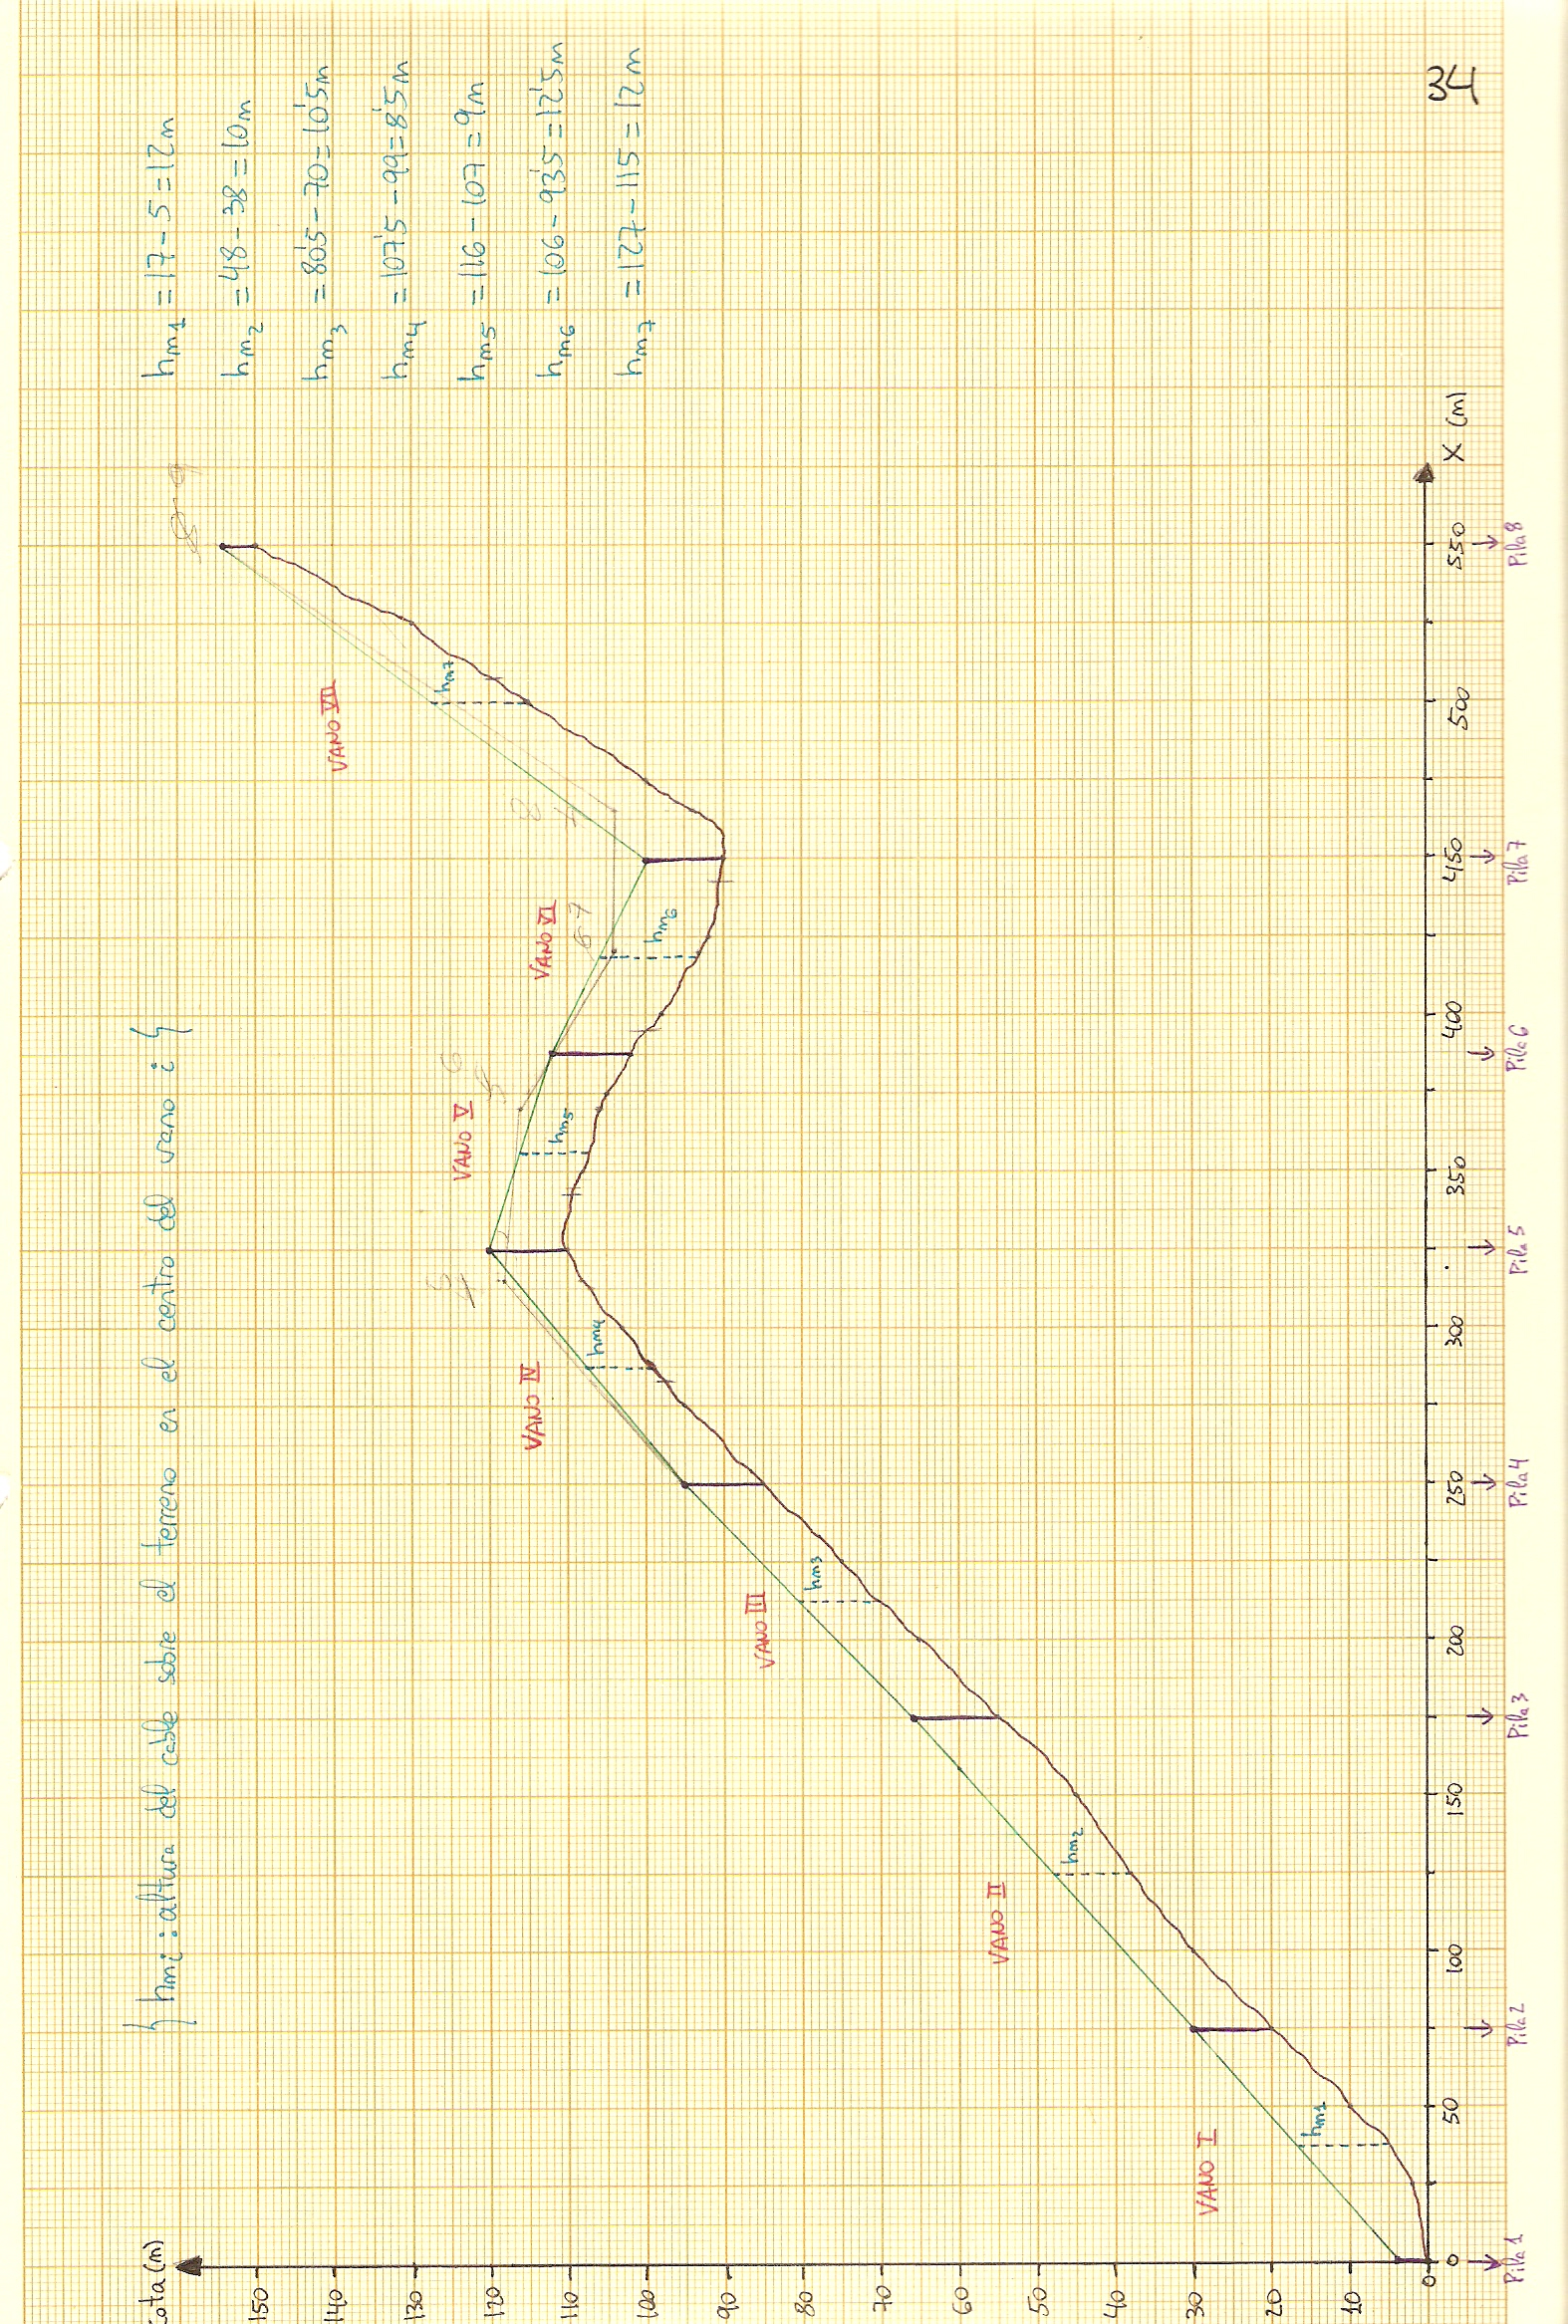
\includegraphics[scale=.75]{Perfil.jpg}
\caption{Perfil final de la instalación, incluyendo la ubicación y altura de cada una de las pilonas que son necesarias en nuestra instalación.}
\label{perfil}
\end{figure}
\bibliography{Transporte_por_cable}
\bibliographystyle{unsrt}
\end{document}
